\newpage
\section{Tabular Integration by Parts}
    One can use a table to perform repeated integration by parts quickly. Suppose we would like to use integration by parts to change the integral of \(v(x)u^{(4)}(x)\) into boundary terms plus the integral of \(v^{(4)}(x)u(x)\). In the first column, we write \(v(x)\) and its derivatives beneath it. In the second column, we write \(u^(4)(x)\) and its anti-derivatives beneath it. At the end of this process, the table should look as follows.
    \begin{table}[H]
        \centering
        \begin{tabular}{c|c}
            \(v(x)\) & \(u^{(4)}(x)\)\\
            \(v'(x)\) & \(u'''(x)\)\\
            \(v''(x)\) & \(u''(x)\)\\
            \(v'''(x)\) & \(u'(x)\)\\
            \(v^{(4)}(x)\) &\(u(x)\)
        \end{tabular}
    \end{table}
    Next, each row of the left column is given alternating signs, beginning with positive.
    \begin{table}[H]
        \centering
        \begin{tabular}{c|c}
            \(+v(x)\) & \(u^{(4)}(x)\)\\
            \(-v'(x)\) & \(u'''(x)\)\\
            \(+v''(x)\) & \(u''(x)\)\\
            \(-v'''(x)\) & \(u'(x)\)\\
            \(+v^{(4)}(x)\) &\(u(x)\)
        \end{tabular}
    \end{table}
    Next we multiply diagonal terms and add each product.
    \begin{figure}[H]
        \centering
        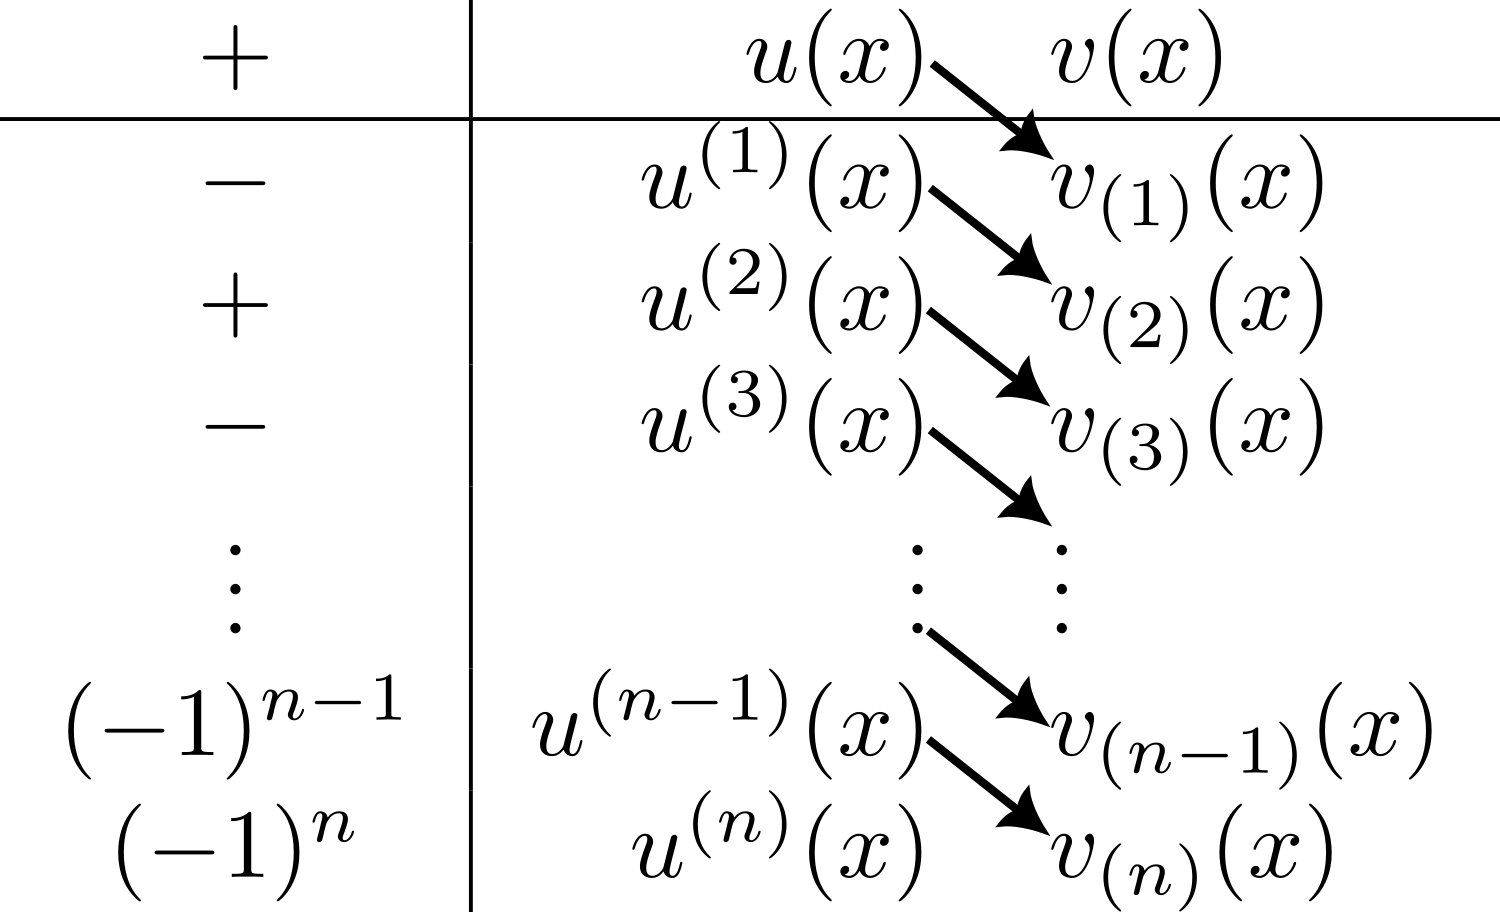
\includegraphics{include/tabular-boundary.png}
    \end{figure}
    These are the boundary terms. Lastly, we multiply the bottom terms together. 
    \begin{figure}[H]
        \centering
        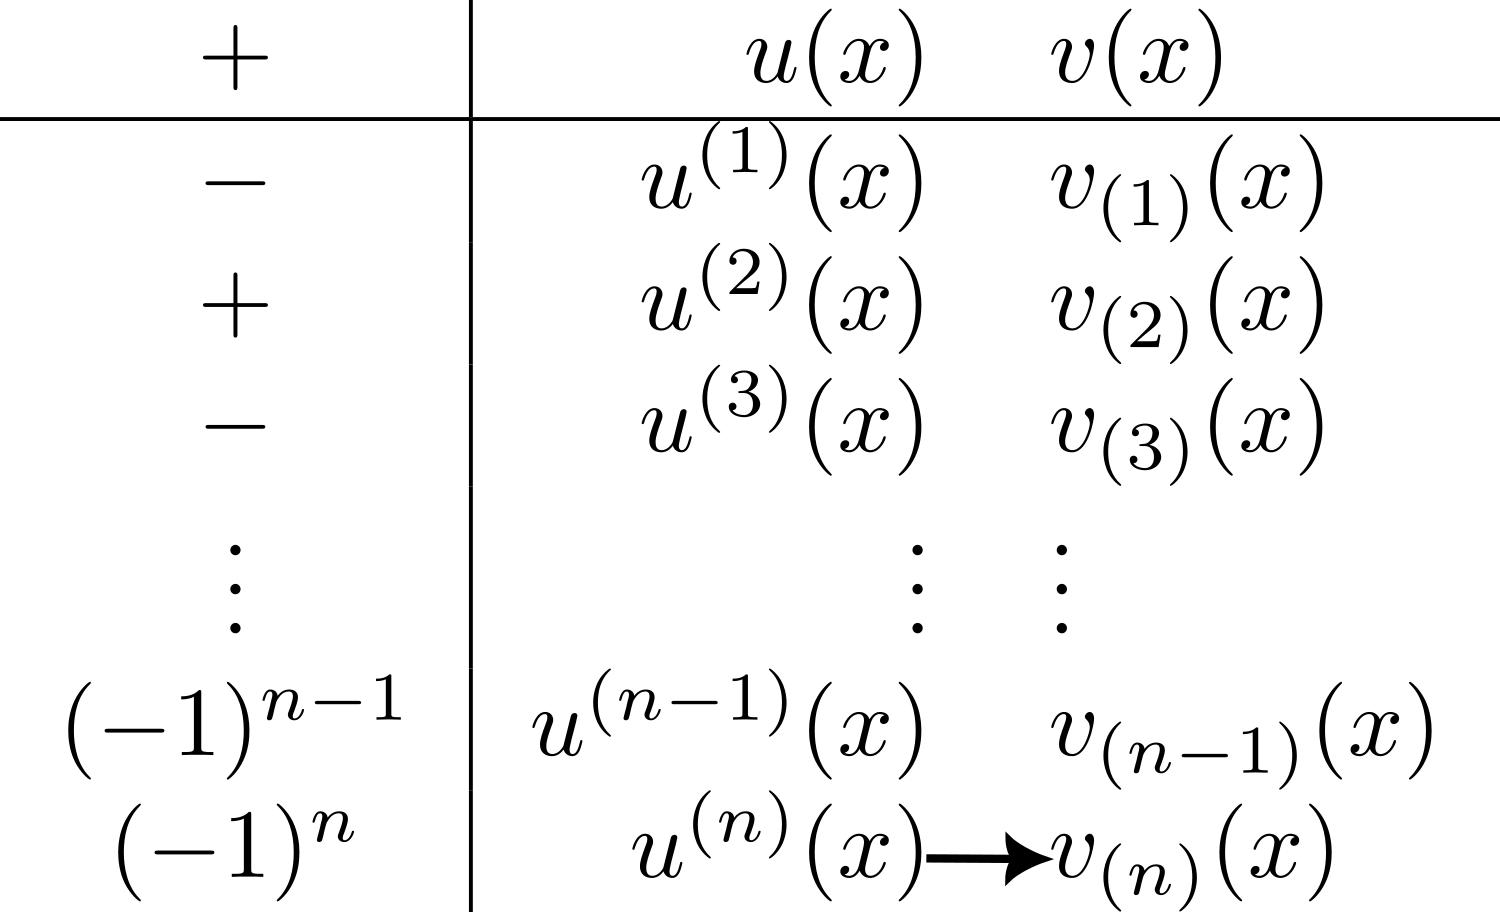
\includegraphics{include/tabular-integrand.png}
    \end{figure}
    This is the integrand. The result at the end of this is 
    \begin{equation}
        \intl v(x)u^{(4)}(x) dx = (v(x)u'''(x) - v'(x)u''(x) + v''(x)u'(x)-v'''(x)u(x))\biggr\rvert_\mathrm{a}^\mathrm{b} + \intl v^{(4)}(x)u(x) dx.
    \end{equation}
\section{The Mean Value Theorem}
    The mean value theorem states that for all \(f:[\lima,\limb]\to \mathbb{R}\) such that \(f\) is continuous on \([\lima,\limb]\), and differentiable on \((\lima, \limb)\), then 
    \begin{equation}
        \exists c \in (\lima, \limb) : f'(\text{c}) = \frac{f(\limb)-f(\lima)}{\limb-\lima}
    \end{equation}
    and thus,
    \begin{equation}
        f'(c)(\limb-\lima) = f(\limb)-f(\lima)
    \end{equation}
    By integrating \(f'(x)\) , we see that
    \begin{equation}
        \begin{split}
            \int_\lima^\limb f'(x) dx &= f(\limb)-f(\lima)\\
            &=f'(\text{c})(\limb-\lima)
        \end{split}
    \end{equation}
\section{Big O Notation}
Big O notation is used to describe the limiting behavior of a function as the argument tends to some value or infinity. By \(f(x)=O(g(x)\) as \(x\to x_0\) we mean that \(\frac{f(x)}{g(x)}\) is bounded as \(x\to x_0\). For example 
\begin{equation}
    \sin 6x = O(1) \text{ as } x\to \inf.
\end{equation}